In this section we will deal with the problem of placing side chains
on the protein and selecting side-chain conformations in a way that
minimizes the number of collisions.

As we mentioned in Section \ref{chap:protein_geometry}, statistical
analysis has shown that each type of amino acid side-chain has a small
set of common conformations \cite{dunbrack2002rotamer}. A side-chain
conformation is a configuration of its $\chi$ angles and is called a
\textit{rotamer}.

There has been developed several \textit{rotamer libraries}
\cite{dunbrack2002rotamer, lovell2000penultimate}, containing lists of
the common rotamers for each side-chain together with a probability of
each of those rotamer occuring in a protein. We have selected to use
the rotamer library made by Dunbrack et al. for the SCWRL side-chain
predictor.

\section{Our approach}

\begin{figure}
	\centering
	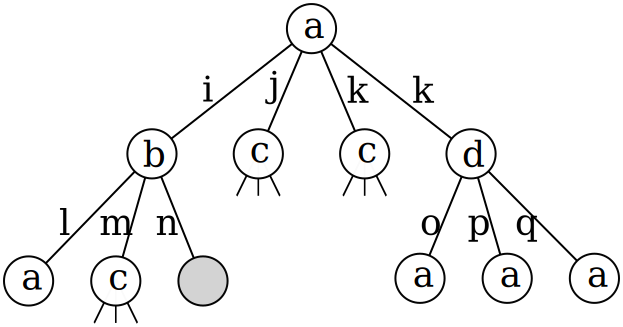
\includegraphics[width=.9\columnwidth]{figures/rotamersearch}
	\caption{woop}
\end{figure}


\section{Related Work}
SCWRL: 
 * Bruger energiberegning i valget af rotamerer
 * Tjekker om par af cysteine amino syrer kan danne disulfid broer


Todo: snak om SCWRL, der tilføjer side-chains på en fastlåst backbone.


%%% Local Variables: 
%%% mode: latex
%%% TeX-master: "rapport"
%%% End: 
